\documentclass[11pt,ignorenonframetext,]{beamer}
\setbeamertemplate{caption}[numbered]
\setbeamertemplate{caption label separator}{: }
\setbeamercolor{caption name}{fg=normal text.fg}
\beamertemplatenavigationsymbolsempty
\usepackage{lmodern}
\usepackage{amssymb,amsmath}
\usepackage{ifxetex,ifluatex}
\usepackage{fixltx2e} % provides \textsubscript
\ifnum 0\ifxetex 1\fi\ifluatex 1\fi=0 % if pdftex
  \usepackage[T1]{fontenc}
  \usepackage[utf8]{inputenc}
\else % if luatex or xelatex
  \ifxetex
    \usepackage{mathspec}
  \else
    \usepackage{fontspec}
  \fi
  \defaultfontfeatures{Ligatures=TeX,Scale=MatchLowercase}
\fi
\usetheme[]{metropolis}
% use upquote if available, for straight quotes in verbatim environments
\IfFileExists{upquote.sty}{\usepackage{upquote}}{}
% use microtype if available
\IfFileExists{microtype.sty}{%
\usepackage{microtype}
\UseMicrotypeSet[protrusion]{basicmath} % disable protrusion for tt fonts
}{}
\newif\ifbibliography
\hypersetup{
            pdftitle={Lecture 18},
            pdfauthor={Colin Rundel},
            pdfborder={0 0 0},
            breaklinks=true}
\urlstyle{same}  % don't use monospace font for urls
\usepackage{color}
\usepackage{fancyvrb}
\newcommand{\VerbBar}{|}
\newcommand{\VERB}{\Verb[commandchars=\\\{\}]}
\DefineVerbatimEnvironment{Highlighting}{Verbatim}{commandchars=\\\{\}}
% Add ',fontsize=\small' for more characters per line
\newenvironment{Shaded}{}{}
\newcommand{\KeywordTok}[1]{\textcolor[rgb]{0.00,0.44,0.13}{\textbf{#1}}}
\newcommand{\DataTypeTok}[1]{\textcolor[rgb]{0.56,0.13,0.00}{#1}}
\newcommand{\DecValTok}[1]{\textcolor[rgb]{0.25,0.63,0.44}{#1}}
\newcommand{\BaseNTok}[1]{\textcolor[rgb]{0.25,0.63,0.44}{#1}}
\newcommand{\FloatTok}[1]{\textcolor[rgb]{0.25,0.63,0.44}{#1}}
\newcommand{\ConstantTok}[1]{\textcolor[rgb]{0.53,0.00,0.00}{#1}}
\newcommand{\CharTok}[1]{\textcolor[rgb]{0.25,0.44,0.63}{#1}}
\newcommand{\SpecialCharTok}[1]{\textcolor[rgb]{0.25,0.44,0.63}{#1}}
\newcommand{\StringTok}[1]{\textcolor[rgb]{0.25,0.44,0.63}{#1}}
\newcommand{\VerbatimStringTok}[1]{\textcolor[rgb]{0.25,0.44,0.63}{#1}}
\newcommand{\SpecialStringTok}[1]{\textcolor[rgb]{0.73,0.40,0.53}{#1}}
\newcommand{\ImportTok}[1]{#1}
\newcommand{\CommentTok}[1]{\textcolor[rgb]{0.38,0.63,0.69}{\textit{#1}}}
\newcommand{\DocumentationTok}[1]{\textcolor[rgb]{0.73,0.13,0.13}{\textit{#1}}}
\newcommand{\AnnotationTok}[1]{\textcolor[rgb]{0.38,0.63,0.69}{\textbf{\textit{#1}}}}
\newcommand{\CommentVarTok}[1]{\textcolor[rgb]{0.38,0.63,0.69}{\textbf{\textit{#1}}}}
\newcommand{\OtherTok}[1]{\textcolor[rgb]{0.00,0.44,0.13}{#1}}
\newcommand{\FunctionTok}[1]{\textcolor[rgb]{0.02,0.16,0.49}{#1}}
\newcommand{\VariableTok}[1]{\textcolor[rgb]{0.10,0.09,0.49}{#1}}
\newcommand{\ControlFlowTok}[1]{\textcolor[rgb]{0.00,0.44,0.13}{\textbf{#1}}}
\newcommand{\OperatorTok}[1]{\textcolor[rgb]{0.40,0.40,0.40}{#1}}
\newcommand{\BuiltInTok}[1]{#1}
\newcommand{\ExtensionTok}[1]{#1}
\newcommand{\PreprocessorTok}[1]{\textcolor[rgb]{0.74,0.48,0.00}{#1}}
\newcommand{\AttributeTok}[1]{\textcolor[rgb]{0.49,0.56,0.16}{#1}}
\newcommand{\RegionMarkerTok}[1]{#1}
\newcommand{\InformationTok}[1]{\textcolor[rgb]{0.38,0.63,0.69}{\textbf{\textit{#1}}}}
\newcommand{\WarningTok}[1]{\textcolor[rgb]{0.38,0.63,0.69}{\textbf{\textit{#1}}}}
\newcommand{\AlertTok}[1]{\textcolor[rgb]{1.00,0.00,0.00}{\textbf{#1}}}
\newcommand{\ErrorTok}[1]{\textcolor[rgb]{1.00,0.00,0.00}{\textbf{#1}}}
\newcommand{\NormalTok}[1]{#1}
\usepackage{graphicx,grffile}
\makeatletter
\def\maxwidth{\ifdim\Gin@nat@width>\linewidth\linewidth\else\Gin@nat@width\fi}
\def\maxheight{\ifdim\Gin@nat@height>\textheight0.8\textheight\else\Gin@nat@height\fi}
\makeatother
% Scale images if necessary, so that they will not overflow the page
% margins by default, and it is still possible to overwrite the defaults
% using explicit options in \includegraphics[width, height, ...]{}
\setkeys{Gin}{width=\maxwidth,height=\maxheight,keepaspectratio}

% Prevent slide breaks in the middle of a paragraph:
\widowpenalties 1 10000
\raggedbottom

\AtBeginPart{
  \let\insertpartnumber\relax
  \let\partname\relax
  \frame{\partpage}
}
\AtBeginSection{
  \ifbibliography
  \else
    \let\insertsectionnumber\relax
    \let\sectionname\relax
    \frame{\sectionpage}
  \fi
}
\AtBeginSubsection{
  \let\insertsubsectionnumber\relax
  \let\subsectionname\relax
  \frame{\subsectionpage}
}

\setlength{\parindent}{0pt}
\setlength{\parskip}{6pt plus 2pt minus 1pt}
\setlength{\emergencystretch}{3em}  % prevent overfull lines
\providecommand{\tightlist}{%
  \setlength{\itemsep}{0pt}\setlength{\parskip}{0pt}}
\setcounter{secnumdepth}{0}

\usepackage{geometry}
\usepackage{graphicx}
\usepackage{amssymb}
\usepackage{color}          	% gives color options
\usepackage{url}		% produces hyperlinks
\usepackage[english]{babel}
\usepackage{colortbl}	% allows for color usage in tables
\usepackage{multirow}	% allows for rows that span multiple rows in tables
\usepackage{xcolor}		% this package has a variety of color options
\usepackage{calc}
\usepackage{multicol}
\usepackage{wrapfig}
\usepackage{textcomp}
\usepackage{bm}
\usepackage{bbm}
\usepackage{setspace}
\usepackage{changepage}
\singlespacing

\usepackage{fontspec}
\newfontfamily\DejaSans{DejaVu Sans}

%%%%%%%%%%%%%%%%
% Small code output
%%%%%%%%%%%%%%%%

%% change fontsize of R code

\makeatletter
\@ifundefined{Shaded}{\newenvironment{Shaded}{}{}}{}
\makeatother


\let\oldShaded\Shaded
\let\endoldShaded\endShaded
\renewenvironment{Shaded}{\footnotesize\begin{spacing}{0.9}\oldShaded}{\endoldShaded\end{spacing}}

%% change fontsize of output
\let\oldverbatim\verbatim
\let\endoldverbatim\endverbatim
\renewenvironment{verbatim}{\footnotesize\begin{spacing}{0.9}\oldverbatim}{\endoldverbatim\end{spacing}}


\newcommand{\tinyoutput}{
  \renewenvironment{Shaded}{\tiny\begin{spacing}{0.9}\oldShaded}{\endoldShaded\end{spacing}}
  \renewenvironment{verbatim}{\tiny\begin{spacing}{0.9}\oldverbatim}{\endoldverbatim\end{spacing}}
}

\newcommand{\scriptoutput}{
  \renewenvironment{Shaded}{\scriptsize\begin{spacing}{0.9}\oldShaded}{\endoldShaded\end{spacing}}
  \renewenvironment{verbatim}{\scriptsize\begin{spacing}{0.9}\oldverbatim}{\endoldverbatim\end{spacing}}
}

\newcommand{\footnoteoutput}{
  \renewenvironment{Shaded}{\footnotesize\begin{spacing}{0.9}\oldShaded}{\endoldShaded\end{spacing}}
  \renewenvironment{verbatim}{\footnotesize\begin{spacing}{0.9}\oldverbatim}{\endoldverbatim\end{spacing}}
}

%\newcommand{\verbatimfont}[1]{\renewcommand{\verbatim@font}{\ttfamily#1}}


%%%%%%%%%%%%%%%%
% Custom Colors
%%%%%%%%%%%%%%%%

\xdefinecolor{oiBlue}{rgb}{0.15, 0.35, 0.55}
\xdefinecolor{gray}{rgb}{0.5, 0.5, 0.5}
\xdefinecolor{darkGray}{rgb}{0.3, 0.3, 0.3}
\xdefinecolor{darkerGray}{rgb}{0.2, 0.2, 0.2}
\xdefinecolor{rubineRed}{rgb}{0.89,0,0.30}
\xdefinecolor{linkCol}{rgb}{0.11,0.49,0.95}	
\xdefinecolor{irishGreen}{rgb}{0,0.60,0}	
\xdefinecolor{darkturquoise}{rgb}{0.44, 0.58, 0.86}
\definecolor{lightGreen}{rgb}{0.533,0.765,0.42}
%\xdefinecolor{hlblue}{rgb}{0.051,0.65,1}
\xdefinecolor{hlblue}{rgb}{ 0.055, 0.639, 0.831}
\definecolor{light}{rgb}{.337,.608,.741}
\definecolor{dark}{rgb}{.337,.608,.741}

\definecolor{cpink}{rgb}{0.93, 0.23, 0.51}

%%%%%%%%%%%%%%%%
% Custom Commands
%%%%%%%%%%%%%%%%

% text colors
\newcommand{\red}[1]{\textit{\textcolor{rubineRed}{#1}}}
\newcommand{\orange}[1]{\textit{\textcolor{orange}{#1}}}
\newcommand{\pink}[1]{\textit{\textcolor{rubineRed!90!white!50}{#1}}}
\newcommand{\green}[1]{\textit{\textcolor{irishGreen}{#1}}}
\newcommand{\blue}[1]{\textit{\textcolor{darkturquoise}{#1}}}
\newcommand{\light}[1]{\textcolor{light}{\textbf{#1}}}
\newcommand{\dark}[1]{\textcolor{dark}{#1}}
\newcommand{\gray}[1]{\textcolor{gray}{#1}}


% links: webURL, webLin, appLink
\newcommand{\webURL}[1]{\urlstyle{same}{\textit{\textcolor{linkCol}{\url{#1}}} }}
\newcommand{\webLink}[2]{\href{#1}{\textcolor{linkCol}{{#2}}}}
\newcommand{\appLink}[2]{\href{#1}{\textcolor{lightGreen!80!black!90}{{#2}}}}

% mail
\newcommand{\mail}[1]{\href{mailto:#1}{\textit{\textcolor{linkCol}{#1}}}}

% highlighting: hl, hlGr, mathhl
\newcommand{\hl}[1]{\textit{\textcolor{hlblue}{#1}}}
\newcommand{\hlGr}[1]{\textit{\textcolor{lightGreen}{#1}}}
\newcommand{\hlRd}[1]{\textit{\textcolor{rubineRed}{#1}}}
\newcommand{\mathhl}[1]{\textcolor{hlblue}{\ensuremath{#1}}}

% example
\newcommand{\ex}[1]{\textcolor{blue}{{{\small (#1)}}}}


\DeclareMathOperator*{\argmin}{arg\,min}
\DeclareMathOperator*{\argmax}{arg\,max}

\title{Lecture 18}
\subtitle{Models for areal data}
\author{Colin Rundel}
\date{03/22/2017}

\begin{document}
\frame{\titlepage}

\section{areal / lattice data}\label{areal-lattice-data}

\begin{frame}{Example - NC SIDS}

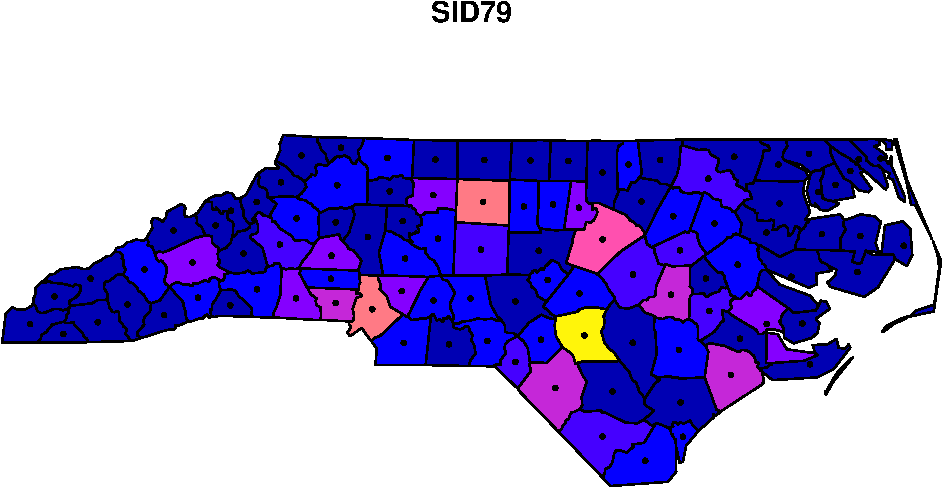
\includegraphics{Lec18_files/figure-beamer/unnamed-chunk-1-1.pdf}

\end{frame}

\begin{frame}[t]{EDA - Moran's I}

If we have observations at \(n\) spatial locations \((s_1, \ldots s_n)\)

\[ I = \frac{n}{\sum_{i=1}^n \sum_{j=1}^n w_{ij}} \frac{\sum_{i=1}^n \sum_{j=1}^n w_{ij} \big(y(s_i)-\bar{y}\big)\big(y(s_j)-\bar{y}\big)}{\sum_{i=1}^n \big(y(s_i) - \bar{y}\big)} \]
where \(\bm{w}\) is a spatial weights matrix.

\pause

\vspace{7mm}

Some properties of Moran's I (when there is no spatial autocorrelation):

\begin{itemize}
\tightlist
\item
  \(E(I) = -1 / (n-1)\)
\end{itemize}

\vspace{2mm}

\begin{itemize}
\tightlist
\item
  \(Var(I) = E(I^2) - E(I)^2 = \text{Something ugly but closed form}\)
\end{itemize}

\vspace{2mm}

\begin{itemize}
\tightlist
\item
  Asymptotically,
  \(\frac{I - E(I)}{\sqrt{Var(I)}} \sim \mathcal{N}(0,1)\)
\end{itemize}

\end{frame}

\begin{frame}[fragile]{NC SIDS \& Moran's I}

Lets start by using an adjacency matrix for \(\bm{w}\) (shared county
borders).

\scriptoutput

\begin{Shaded}
\begin{Highlighting}[]
\NormalTok{morans_I =}\StringTok{ }\ControlFlowTok{function}\NormalTok{(y, w)}
\NormalTok{\{}
\NormalTok{  n =}\StringTok{ }\KeywordTok{length}\NormalTok{(y)}
\NormalTok{  y_bar =}\StringTok{ }\KeywordTok{mean}\NormalTok{(y)}
\NormalTok{  num =}\StringTok{ }\KeywordTok{sum}\NormalTok{(w }\OperatorTok{*}\StringTok{ }\NormalTok{(y}\OperatorTok{-}\NormalTok{y_bar) }\OperatorTok\StringTok{ }\KeywordTok{t}\NormalTok{(y}\OperatorTok{-}\NormalTok{y_bar))  }
\NormalTok{  denom =}\StringTok{ }\KeywordTok{sum}\NormalTok{( (y}\OperatorTok{-}\NormalTok{y_bar)}\OperatorTok{^}\DecValTok{2}\NormalTok{ )}
\NormalTok{  (n}\OperatorTok{/}\KeywordTok{sum}\NormalTok{(w)) }\OperatorTok{*}\StringTok{ }\NormalTok{(num}\OperatorTok{/}\NormalTok{denom)}
\NormalTok{\}}

\KeywordTok{morans_I}\NormalTok{(}\DataTypeTok{y =}\NormalTok{ nc}\OperatorTok{$}\NormalTok{SID74, }\DataTypeTok{w =} \DecValTok{1}\OperatorTok{*}\KeywordTok{st_touches}\NormalTok{(nc, }\DataTypeTok{sparse=}\OtherTok{FALSE}\NormalTok{))}
\NormalTok{## [1] 0.119089}


\KeywordTok{library}\NormalTok{(ape)}
\KeywordTok{Moran.I}\NormalTok{(nc}\OperatorTok{$}\NormalTok{SID74, }\DataTypeTok{weight =} \DecValTok{1}\OperatorTok{*}\KeywordTok{st_touches}\NormalTok{(nc, }\DataTypeTok{sparse=}\OtherTok{FALSE}\NormalTok{)) }\OperatorTok\StringTok{ }\KeywordTok{str}\NormalTok{()}
\NormalTok{## List of 4}
\NormalTok{##  $ observed: num 0.148}
\NormalTok{##  $ expected: num -0.0101}
\NormalTok{##  $ sd      : num 0.0627}
\NormalTok{##  $ p.value : num 0.0118}
\end{Highlighting}
\end{Shaded}

\end{frame}

\begin{frame}[t]{EDA - Geary's C}

Like Moran's I, if we have observations at \(n\) spatial locations
\((s_1, \ldots s_n)\)

\[ C = \frac{n-1}{2\sum_{i=1}^n \sum_{j=1}^n w_{ij}} \frac{\sum_{i=1}^n \sum_{j=1}^n w_{ij} \big(y(s_i)-y(s_j)\big)^2}{\sum_{i=1}^n \big(y(s_i) - \bar{y}\big)} \]
where \(\bm{w}\) is a spatial weights matrix.

\pause

\vspace{7mm}

Some properties of Geary's C:

\begin{itemize}
\tightlist
\item
  \(0 < C < 2\)

  \begin{itemize}
  \tightlist
  \item
    If \(C \approx 1\) then no spatial autocorrelation
  \item
    If \(C > 1\) then negative spatial autocorrelation
  \item
    If \(C < 1\) then positive spatial autocorrelation
  \end{itemize}
\item
  Geary's C is inversely related to Moran's I
\end{itemize}

\end{frame}

\begin{frame}[fragile,t]{NC SIDS \& Geary's C}

Again using an adjacency matrix for \(\bm{w}\) (shared county borders).

\scriptoutput

\begin{Shaded}
\begin{Highlighting}[]
\NormalTok{gearys_C =}\StringTok{ }\ControlFlowTok{function}\NormalTok{(y, w)}
\NormalTok{\{}
\NormalTok{  n =}\StringTok{ }\KeywordTok{length}\NormalTok{(y)}
\NormalTok{  y_bar =}\StringTok{ }\KeywordTok{mean}\NormalTok{(y)}
\NormalTok{  y_i =}\StringTok{ }\NormalTok{y }\OperatorTok\StringTok{ }\KeywordTok{t}\NormalTok{(}\KeywordTok{rep}\NormalTok{(}\DecValTok{1}\NormalTok{,n))}
\NormalTok{  y_j =}\StringTok{ }\KeywordTok{t}\NormalTok{(y_i)}
\NormalTok{  num =}\StringTok{ }\KeywordTok{sum}\NormalTok{(w }\OperatorTok{*}\StringTok{ }\NormalTok{(y_i}\OperatorTok{-}\NormalTok{y_j)}\OperatorTok{^}\DecValTok{2}\NormalTok{)  }
\NormalTok{  denom =}\StringTok{ }\KeywordTok{sum}\NormalTok{( (y}\OperatorTok{-}\NormalTok{y_bar)}\OperatorTok{^}\DecValTok{2}\NormalTok{ )}
\NormalTok{  ((n}\OperatorTok{-}\DecValTok{1}\NormalTok{)}\OperatorTok{/}\NormalTok{(}\DecValTok{2}\OperatorTok{*}\KeywordTok{sum}\NormalTok{(w))) }\OperatorTok{*}\StringTok{ }\NormalTok{(num}\OperatorTok{/}\NormalTok{denom)}
\NormalTok{\}}

\KeywordTok{gearys_C}\NormalTok{(}\DataTypeTok{y =}\NormalTok{ nc}\OperatorTok{$}\NormalTok{SID74, }\DataTypeTok{w =} \DecValTok{1}\OperatorTok{*}\KeywordTok{st_touches}\NormalTok{(nc, }\DataTypeTok{sparse=}\OtherTok{FALSE}\NormalTok{))}
\NormalTok{## [1] 0.8898868}
\end{Highlighting}
\end{Shaded}

\end{frame}

\begin{frame}[fragile]{Spatial Correlogram}

\scriptoutput

\begin{Shaded}
\begin{Highlighting}[]
\NormalTok{d =}\StringTok{ }\NormalTok{nc }\OperatorTok\StringTok{ }\KeywordTok{st_centroid}\NormalTok{() }\OperatorTok\StringTok{ }\KeywordTok{st_distance}\NormalTok{() }\OperatorTok\StringTok{ }\KeywordTok{strip_class}\NormalTok{()}
\NormalTok{breaks =}\StringTok{ }\KeywordTok{seq}\NormalTok{(}\DecValTok{0}\NormalTok{, }\KeywordTok{max}\NormalTok{(d), }\DataTypeTok{length.out =} \DecValTok{21}\NormalTok{)}
\NormalTok{d_cut =}\StringTok{ }\KeywordTok{cut}\NormalTok{(d, breaks)}

\NormalTok{adj_mats =}\StringTok{ }\KeywordTok{map}\NormalTok{(}
  \KeywordTok{levels}\NormalTok{(d_cut), }
  \ControlFlowTok{function}\NormalTok{(l) }
\NormalTok{  \{}
\NormalTok{    (d_cut }\OperatorTok{==}\StringTok{ }\NormalTok{l) }\OperatorTok
\StringTok{      }\KeywordTok{matrix}\NormalTok{(}\DataTypeTok{ncol=}\DecValTok{100}\NormalTok{) }\OperatorTok
\StringTok{      `}\DataTypeTok{diag<-}\StringTok{`}\NormalTok{(}\DecValTok{0}\NormalTok{)}
\NormalTok{  \}}
\NormalTok{)}

\NormalTok{d =}\StringTok{ }\KeywordTok{data_frame}\NormalTok{(}
  \DataTypeTok{dist   =}\NormalTok{ breaks[}\OperatorTok{-}\DecValTok{1}\NormalTok{],}
  \DataTypeTok{morans =} \KeywordTok{map_dbl}\NormalTok{(adj_mats, morans_I, }\DataTypeTok{y =}\NormalTok{ nc}\OperatorTok{$}\NormalTok{SID74),}
  \DataTypeTok{gearys =} \KeywordTok{map_dbl}\NormalTok{(adj_mats, gearys_C, }\DataTypeTok{y =}\NormalTok{ nc}\OperatorTok{$}\NormalTok{SID74)}
\NormalTok{)}
\end{Highlighting}
\end{Shaded}

\end{frame}

\begin{frame}{}

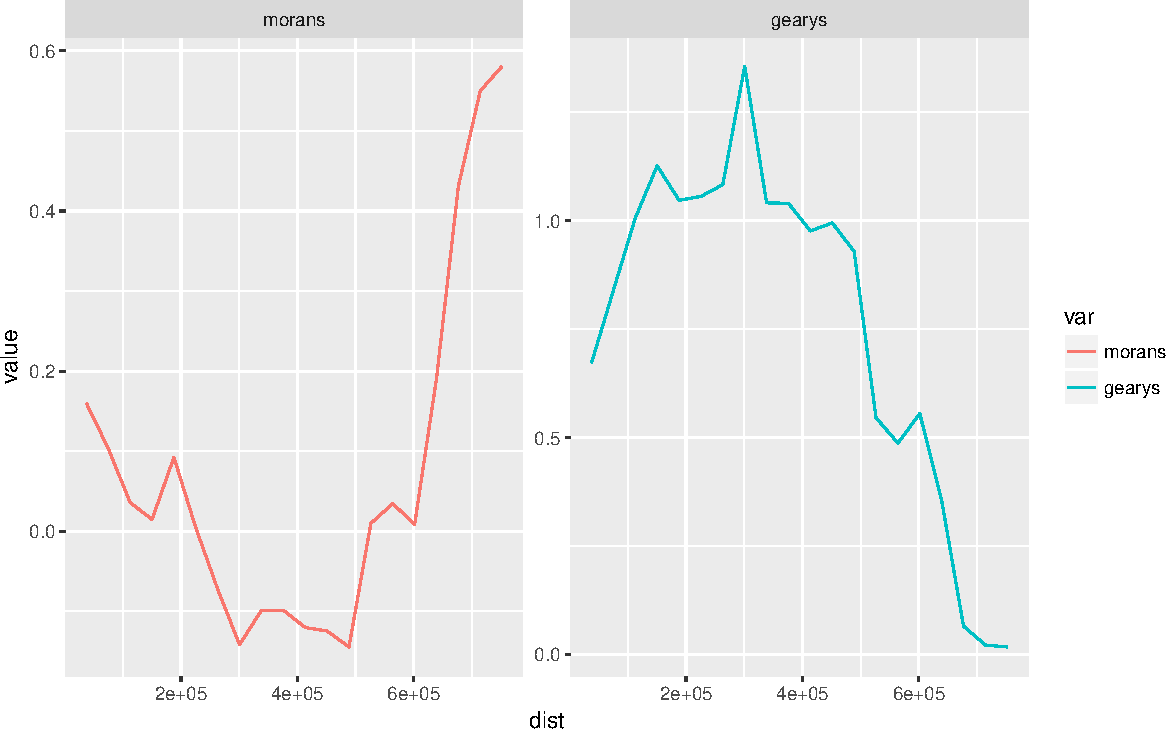
\includegraphics{Lec18_files/figure-beamer/unnamed-chunk-5-1.pdf}

\end{frame}

\begin{frame}{}

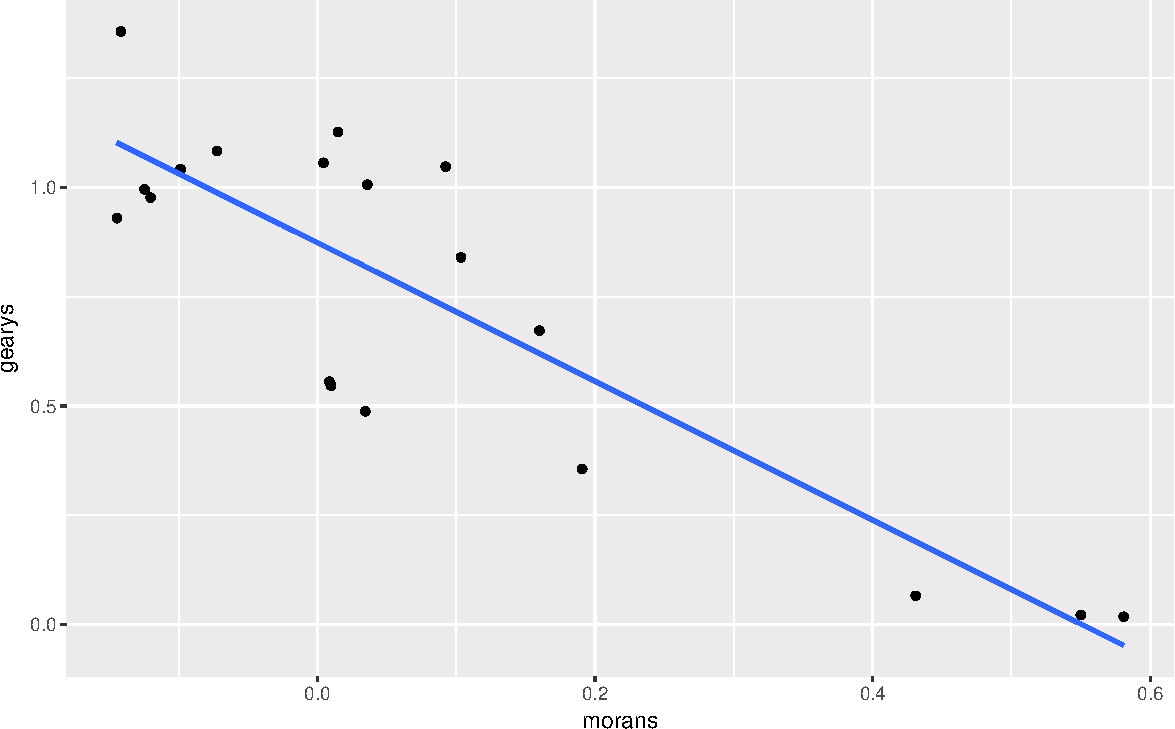
\includegraphics{Lec18_files/figure-beamer/unnamed-chunk-6-1.pdf}

\end{frame}

\section{Autoregressive Models}\label{autoregressive-models}

\begin{frame}[t]{AR Models - Time}

Lets just focus on the simplest case, an \(AR(1)\) process

\[ y_t = \delta + \phi \, y_{t-1} + w_t \]

where \(w_t \sim \mathcal{N}(0,\sigma^2)\) and \(|\phi| < 1\), then

\[
\begin{aligned}
E(y_t) &= \frac{\delta}{1-\phi} \\
Var(y_t) &= \frac{\sigma^2}{1-\phi}
\end{aligned}
\]

\end{frame}

\begin{frame}[t]{AR Models - Time - Joint Distribution}

Previously we saw that an \(AR(1)\) model can be represented using a
multivariate normal distribution

\[
\begin{pmatrix}
y_1 \\ y_2 \\ \vdots \\ y_n
\end{pmatrix}
\sim \mathcal{N} \begin{pmatrix}
\frac{\delta}{1-\phi} \begin{pmatrix}1\\ 1\\ \vdots\\ 1\end{pmatrix},~
\frac{\sigma^2}{1-\phi}
\begin{pmatrix}
1      & \phi   & \cdots & \phi^{n-1} \\
\phi   & 1      & \cdots & \phi^{n-2} \\
\vdots & \vdots & \ddots & \vdots     \\
\phi^{n-1} & \phi^{n-2}  & \cdots & 1 \\
\end{pmatrix}
\end{pmatrix}
\]

\pause

\vspace{4mm}

In writing down the likelihood we also saw that an \(AR(1)\) is 1st
order Markovian,

\[ \begin{aligned}
f(y_1, \ldots, y_n) 
  &= f(y_1) \, f(y_2 | y_1) \,  f(y_3|y_2,y_1) \,\cdots\, f(y_n|y_{n-1},y_{n-2},\ldots,y_1) \\
  &= f(y_1) \, f(y_2 | y_1) \,  f(y_3|y_2) \,\cdots\, f(y_n|y_{n-1})
\end{aligned} \]

\end{frame}

\begin{frame}{Competing Definitions for \(y_t\)}

\Large

\[ y_t = \delta + \phi \, y_{t-1} + w_t \]

\vspace{2mm}

\begin{center}vs.\end{center}

\vspace{2mm}

\[ y_t | y_{t-1} \sim \mathcal{N}(\delta + \phi \, y_{t-1},~\sigma^2) \]

\pause

\vspace{3mm}

In the case of time, both of these definitions result in the same
multivariate distribution for \(\bm{y}\).

\end{frame}

\begin{frame}[t]{AR in Space}

\vspace{4mm}

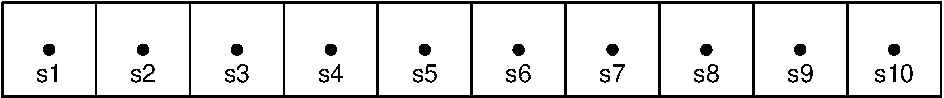
\includegraphics{Lec18_files/figure-beamer/unnamed-chunk-7-1.pdf}

\pause

Even in the simplest spatial case there is no clear / unique ordering,
\footnotesize
\[ \begin{aligned}
f\big(y(s_1), \ldots, y(s_{10})\big) 
  &= f\big(y(s_1)\big) \, f\big(y(s_2) | y(s_1)\big) \, \cdots \, f\big(y(s_{10} | y(s_{9}),y(s_{8}),\ldots,y(s_1)\big)  \\
  &= f\big(y(s_{10})\big) \, f\big(y(s_9) | y(s_{10})\big) \, \cdots \, f\big(y(s_{1} | y(s_{2}),y(s_{3}),\ldots,y(s_{10})\big)  \\
  &= ~?
\end{aligned} \] \normalsize

\pause

Instead we need to think about things in terms of their neighbors /
neighborhoods. We will define \(N(s_i)\) to be the set of neighbors of
location \(s_i\).

\begin{itemize}
\item
  If we define the neighborhood based on ``touching'' then
  \(N(s_3) = \{s_2, s_4\}\)
\item
  If we use distance within 2 units then
  \(N(s_3) = \{s_1,s_2,s_3,s_4\}\)
\item
  etc.
\end{itemize}

\end{frame}

\begin{frame}[t]{Defining the Spatial AR model}

Here we will consider a simple average of neighboring observations, just
like with the temporal AR model we have two options in terms of defining
the autoregressive process,

\begin{itemize}
\tightlist
\item
  Simultaneous Autogressve (SAR)
\end{itemize}

\[ y(s) = \delta + \phi \frac{1}{|N(s)|}\sum_{s' \in N(s)} y(s') + \mathcal{N}(0,\sigma^2) \]

\begin{itemize}
\tightlist
\item
  Conditional Autoregressive (CAR)
\end{itemize}

\[ y(s)|\bm{y}_{-s} \sim \mathcal{N}\left(\delta + \phi \frac{1}{|N(s)|}\sum_{s' \in N(s)} y(s'),~ \sigma^2 \right) \]

\end{frame}

\begin{frame}[t]{Simultaneous Autogressve (SAR)}

\vspace{-3mm}

Using
\[ y(s) = \delta + \phi \frac{1}{|N(s)|}\sum_{s' \in N(s)} y(s') + \mathcal{N}(0,\sigma^2) \]
we want to find the distribution of
\(\bm{y} = \Big(y(s_1),\, y(s_2),\,\ldots,\,y(s_n)\Big)^t\).

\pause

\vspace{5mm}

First we need to define a weight matrix \(\bm W\) where \[ 
\{\bm W\}_{ij} = \begin{cases}
1/|N(s_i)| & \text{if $j \in N(s_i)$} \\
0        & \text{otherwise}
\end{cases}
\]

\pause

then we can write \(\bm y\) as follows,
\[ \bm{y} = \bm{\delta} + \phi \, \bm{W} \, \bm{y} + \bm{\epsilon} \]
where \[ \bm\epsilon \sim \mathcal{N}(0,\sigma^2 \, \bm{I}) \]

\end{frame}

\begin{frame}[t]{A toy example}

\begin{tabular}{c}
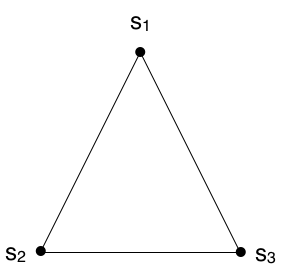
\includegraphics[width=0.3\textwidth]{figs/triangle_adj.png} \\
~\\
~\\
$\bm{W} = \begin{bmatrix}
0   & 1/2 & 1/2 \\
1/2 & 0   & 1/2 \\
1/2 & 1/2 & 0   \\
\end{bmatrix}$
\end{tabular}

\end{frame}

\begin{frame}[t]{Back to SAR}

\[ \bm{y} = \bm{\delta} + \phi \, \bm{W} \, \bm{y} + \bm{\epsilon} \]

\end{frame}

\begin{frame}[t]{Conditional Autogressve (CAR)}

This is a bit trickier, in the case of the temporal AR process we
actually went from joint distribution \(\to\) conditional distributions
(which we were then able to simplify).

\vspace{3mm}

Since we don't have a natural ordering we can't get away with this (at
least not easily).

\vspace{3mm}

Going the other way, conditional distributions \(\to\) joint
distribution is difficult because it is possible to specify conditional
distributions that lead to an improper joint distribution.

\end{frame}

\begin{frame}[t]{Brook's Lemma}

For sets of observations \(\bm{x}\) and \(\bm{y}\) where
\(p(x) > 0~~\forall ~ x\in\bm{x}\) and
\(p(y) > 0~~\forall ~ y\in\bm{y}\) then

\[\begin{aligned}
\frac{p(\bm{y})}{p(\bm{x})} 
  &= \prod_{i=1}^n \frac{p(y_i ~|~ y_1,\ldots,y_{i-1},x_{i+1},\ldots,x_n)}{p(x_i ~|~ x_1,\ldots,x_{i-1},y_{i+1},\ldots,y_n)} \\
  &= \prod_{i=1}^n \frac{p(y_i ~|~ x_1,\ldots,x_{i-1},y_{i+1},\ldots,y_n)}{p(x_i ~|~ y_1,\ldots,y_{i-1},x_{i+1},\ldots,x_n)} \\
\end{aligned}\]

\end{frame}

\begin{frame}{A simplified example}

Let \(\bm{y} = (y_1,y_2)\) and \(\bm{x} = (x_1,x_2)\) then we can derive
Brook's Lemma for this case,

\[ \begin{aligned}
p (y_1,y_2) 
  &= p(y_1 | y_2) p(y_2) \\
  &= p(y_1 | y_2) \frac{p(y_2|x_1) \, p(x_1)}{p(x_1|y_2)} = \frac{p(y_1 | y_2)}{p(x_1 | y_2)} p(y_2|x_1) \, p(x_1) \\
  & = \frac{p(y_1 | y_2)}{p(x_1 | y_2)} p(y_2|x_1) \, p(x_1) \left(\frac{p(x_2|x_1)}{p(x_2|x_1)}\right) \\
  & = \frac{p(y_1 | y_2)}{p(x_1 | y_2)} \frac{p(y_2|x_1)}{p(x_2|x_1)} \, p(x_1,x_2) \\
\\
\frac{p (y_1,y_2) }{p(x_1,x_2)} 
  & = \frac{p(y_1 | y_2)}{p(x_1 | y_2)} \frac{p(y_2|x_1)}{p(x_2|x_1)}
\end{aligned} \]

\end{frame}

\begin{frame}[t]{Utility?}

Lets repeat that last example but consider the case where
\(\bm{y} = (y_1,y_2)\) but now we let \(\bm{x} = (y_1=0,y_2=0)\)

\[ \begin{aligned}
\frac{p (y_1,y_2) }{p(x_1,x_2)} 
  &= \frac{p (y_1,y_2) }{p(y_1=0,y_2=0)}  \\
\\
p(y_1,y_2) &= \frac{p(y_1 | y_2)}{p(y_1=0 | y_2)} \frac{p(y_2|y_1=0)}{p(y_2=0|y_1=0)} ~ p(y_1=0,y_2=0) \\
\\
p(y_1,y_2) 
  &\propto \frac{p(y_1 | y_2) ~ p(y_2|y_1=0) }{ p(y_1=0 | y_2)} \\
  &\propto \frac{p(y_2 | y_1) ~ p(y_1|y_2=0) }{ p(y_2=0 | y_1)}
\end{aligned} \]

\end{frame}

\begin{frame}[t]{As applied to a \textbf{simple} CAR}

\begin{center}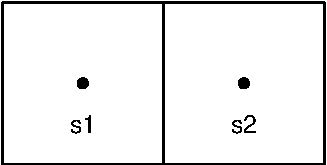
\includegraphics[width=0.2\textwidth]{Lec18_files/figure-beamer/unnamed-chunk-8-1} \end{center}

\scriptsize
\[ \begin{aligned}
y(s_1) | y(s_2) \sim \mathcal{N}(\phi W_{12}\, y(s_2), \sigma^2) \\
y(s_2) | y(s_1) \sim \mathcal{N}(\phi W_{21}\, y(s_1), \sigma^2)
\end{aligned}\]

\pause

\[\begin{aligned}
p\big(y(s_1),y(s_2)\big) 
  &\propto \frac{p\big(y(s_1) | y(s_2)\big) ~ p\big(y(s_2)|y(s_1)=0\big)}{p\big(y(s_1)=0|y(s_2)\big)}\\
  &\propto 
    \frac{
      \exp\left(-\frac{1}{2\sigma^2}\left(y(s_1)-\phi \, W_{12} \, y(s_2)\right)^2\right)
      \exp\left(-\frac{1}{2\sigma^2}\left(y(s_2)-\phi \, W_{21} \, 0\right)^2\right) 
    }{
      \exp\left(-\frac{1}{2\sigma^2}\left(0-\phi W_{12} y(s_2)\right)^2 \right)
    }\\
  &\propto \exp\left(-\frac{1}{2\sigma^2}\left(\left(y(s_1)-\phi \, W_{12} \, y(s_2)\right)^2 + y(s_2)^2- (\phi W_{12} y(s_2))^2\right)\right) \\
  &\propto \exp\left(-\frac{1}{2\sigma^2}\left(y(s_1)^2-2\phi \, W_{12} \, y(s_1)\,y(s_2) + y(s_2)^2\right)\right) \\
  &\propto \exp\left(-\frac{1}{2\sigma^2} (\bm{y}-0)
    \begin{pmatrix} 
    1 & -\phi W_{12} \\
    -\phi W_{12} & 1
    \end{pmatrix}
    (\bm{y}-0)^{t}
  \right)
\end{aligned}\]

\end{frame}

\begin{frame}{Implicatiomns for \(\bm{y}\)}

\vspace{-3mm}

\[ \bm{\mu} = 0 \]

\[
\begin{aligned}
\bm{\Sigma}^{-1} &= \frac{1}{\sigma^2}
  \begin{pmatrix} 
    1 & -\phi W_{12} \\
    -\phi W_{12} & 1
  \end{pmatrix} \\
  &= \frac{1}{\sigma^2}(\bm{I} - \phi \, \bm{W})
\end{aligned}
\]

\[
\Sigma = \sigma^2(\bm{I} - \phi \, \bm{W})^{-1}
\]

\pause

we can then conclude that for \(\bm{y} = (y(s_1),~y(s_2))^t\),

\[
\bm{y} \sim \mathcal{N}\left(
\bm{0}, ~
\sigma^2 (\bm{I} - \phi \, \bm{W})^{-1}
\right)
\]

which generalizes for all mean 0 CAR models.

\end{frame}

\begin{frame}{General Proof}

Let \(\bm{y} = (y(s_1),\ldots,y(s_n))\) and
\(\bm{0} = (y(s_1) = 0, \ldots, y(s_n)=0)\) then by Brook's lemma,

\scriptsize

\[\begin{aligned}
\frac{p(\bm{y})}{p(\bm{0})} 
  &= \prod_{i=1}^n \frac{p(y_i|y_1,\ldots,y_{i-1},0_{i+1},\ldots,0_{n})}{p(0_i|y_1,\ldots,y_{i-1},0_{i+1},\ldots,0_{n})} \\
  &= \prod_{i=1}^n 
    \frac{
      \exp\left(-\frac{1}{2\sigma^2} \left(y_i - \phi \sum_{j<i} W_{ij} \, y_j - \phi \sum_{j>i} 0_j \right)^2 \right)
    }{
      \exp\left(-\frac{1}{2\sigma^2} \left(0_i - \phi \sum_{j<i} W_{ij} \, y_j - \phi \sum_{j>i} 0_j \right)^2 \right)
    } \\
  &= \exp\left(-\frac{1}{2\sigma^2} \sum_{i=1}^n \left(y_i - \phi \sum_{j<i} W_{ij} \, y_j\right)^2 + \frac{1}{2\sigma^2} \sum_{i=1}^n \left( \phi \sum_{j<i} W_{ij} \, y_j \right)^2 \right) \\
  &= \exp\left(-\frac{1}{2\sigma^2} \sum_{i=1}^n y_i^2 - 2 \phi y_i \,\sum_{j<i} W_{ij} \, y_j \right) \\
  &= \exp\left(-\frac{1}{2\sigma^2} \sum_{i=1}^n y_i^2 - \phi \sum_{i=1}^n \sum_{j=1}^n y_i \, W_{ij} \, y_j \right) \quad \mathit{\big(\text{if } W_{ij} = W_{ji}\big)} \\
  &= \exp\left(-\frac{1}{2\sigma^2} \bm{y}^t (\bm{I} - \phi \bm{W}) \bm{y}  \right)
\end{aligned}\]

\end{frame}

\begin{frame}{CAR vs SAR}

\begin{itemize}
\tightlist
\item
  Simultaneous Autogressve (SAR)
\end{itemize}

\[ y(s) = \phi \sum_{s'} \frac{W_{s\,s'}}{W_{s\,\boldsymbol{\cdot}}} y(s') + \epsilon \]

\[ \bm{y} \sim \mathcal{N}(0,~\sigma^2 \, ((\bm{I}-\phi \bm{W})^{-1}) ((\bm{I}-\phi \bm{W})^{-1})^t )\]

\begin{itemize}
\tightlist
\item
  Conditional Autoregressive (CAR)
\end{itemize}

\[ y(s)|\bm{y}_{-s} \sim \mathcal{N}\left(\sum_{s'} \frac{W_{s\,s'}}{W_{s\,\boldsymbol{\cdot}}} y(s'),~ \sigma^2 \right) \]

\[ \bm{y} \sim \mathcal{N}(0,~\sigma^2 \, (\bm{I}-\phi \bm{W})^{-1})\]

\end{frame}

\begin{frame}{Generalization}

\begin{itemize}
\item
  Adopting different weight matrices, \(\bm{W}\)

  \begin{itemize}
  \item
    Between SAR and CAR model we move to a generic weight matrix
    definition (beyond average of nearest neighbors)
  \item
    In time we varied \(p\) in the \(AR(p)\) model, in space we adjust
    the weight matrix.
  \item
    In general having a symmetric W is helpful, but not required
  \end{itemize}
\item
  More complex Variance (beyond \(\sigma^2 \, I\))

  \begin{itemize}
  \item
    \(\sigma^2\) can be a vector (differences between areal locations)
  \item
    E.g. since areal data tends to be aggregated - adjust variance based
    on sample size
  \end{itemize}
\end{itemize}

\end{frame}

\end{document}
